
\documentclass{standalone}
\usepackage{tikz}
\begin{document}
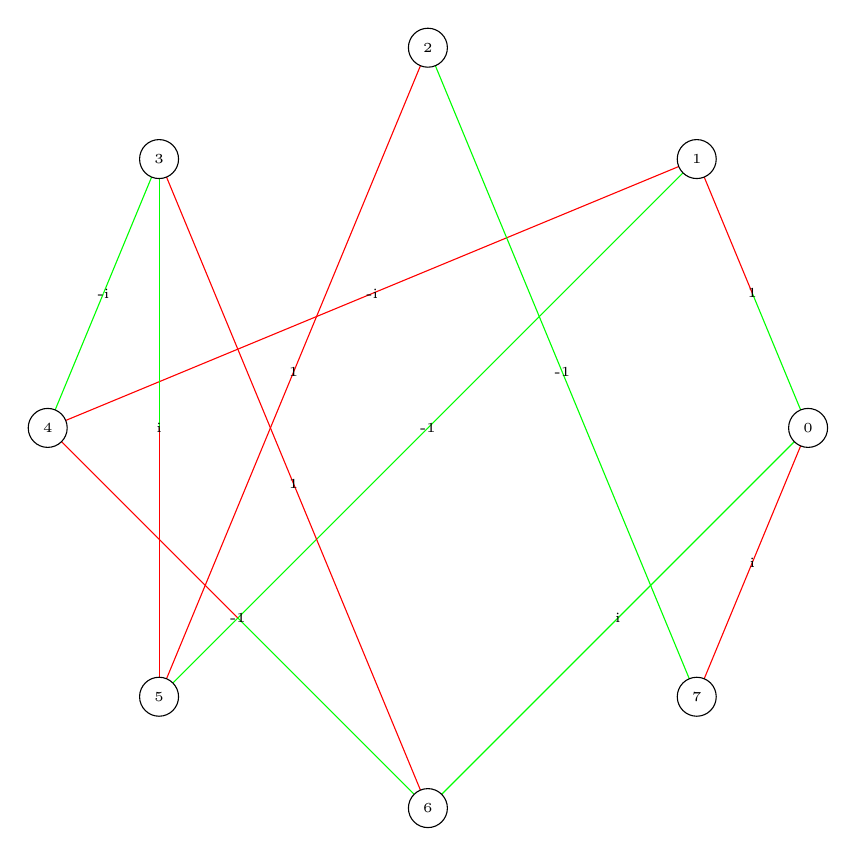
\begin{tikzpicture}
\tikzstyle{every node}=[font=\tiny]
\draw [style=thin, color=green] (4.82842712474619,0.0) to (4.121320343559642,1.7071067811865472);
\draw [style=thin, color=red] (4.121320343559642,1.7071067811865472) to (3.414213562373095,3.4142135623730945);
\node [style=circle, draw=none] at (4.121320343559642,1.7071067811865472) {1};
\draw [style=thin, color=green] (4.82842712474619,0.0) to (2.4142135623730945,-2.414213562373095);
\draw [style=thin, color=green] (2.4142135623730945,-2.414213562373095) to (-8.869676734855019e-16,-4.82842712474619);
\node [style=circle, draw=none] at (2.4142135623730945,-2.414213562373095) {i};
\draw [style=thin, color=red] (4.82842712474619,0.0) to (4.121320343559642,-1.707106781186548);
\draw [style=thin, color=red] (4.121320343559642,-1.707106781186548) to (3.414213562373094,-3.414213562373096);
\node [style=circle, draw=none] at (4.121320343559642,-1.707106781186548) {i};
\draw [style=thin, color=red] (3.414213562373095,3.4142135623730945) to (-0.7071067811865475,1.7071067811865475);
\draw [style=thin, color=red] (-0.7071067811865475,1.7071067811865475) to (-4.82842712474619,5.913117823236679e-16);
\node [style=circle, draw=none] at (-0.7071067811865475,1.7071067811865475) {-i};
\draw [style=thin, color=green] (3.414213562373095,3.4142135623730945) to (-4.440892098500626e-16,0.0);
\draw [style=thin, color=green] (-4.440892098500626e-16,0.0) to (-3.414213562373096,-3.4142135623730945);
\node [style=circle, draw=none] at (-4.440892098500626e-16,0.0) {-1};
\draw [style=thin, color=red] (2.9565589116183395e-16,4.82842712474619) to (-1.7071067811865477,0.7071067811865477);
\draw [style=thin, color=red] (-1.7071067811865477,0.7071067811865477) to (-3.414213562373096,-3.4142135623730945);
\node [style=circle, draw=none] at (-1.7071067811865477,0.7071067811865477) {1};
\draw [style=thin, color=green] (2.9565589116183395e-16,4.82842712474619) to (1.7071067811865472,0.707106781186547);
\draw [style=thin, color=green] (1.7071067811865472,0.707106781186547) to (3.414213562373094,-3.414213562373096);
\node [style=circle, draw=none] at (1.7071067811865472,0.707106781186547) {-1};
\draw [style=thin, color=green] (-3.4142135623730945,3.414213562373095) to (-4.121320343559642,1.7071067811865477);
\draw [style=thin, color=green] (-4.121320343559642,1.7071067811865477) to (-4.82842712474619,5.913117823236679e-16);
\node [style=circle, draw=none] at (-4.121320343559642,1.7071067811865477) {-i};
\draw [style=thin, color=green] (-3.4142135623730945,3.414213562373095) to (-3.414213562373095,2.220446049250313e-16);
\draw [style=thin, color=red] (-3.414213562373095,2.220446049250313e-16) to (-3.414213562373096,-3.4142135623730945);
\node [style=circle, draw=none] at (-3.414213562373095,2.220446049250313e-16) {i};
\draw [style=thin, color=red] (-3.4142135623730945,3.414213562373095) to (-1.7071067811865477,-0.7071067811865475);
\draw [style=thin, color=red] (-1.7071067811865477,-0.7071067811865475) to (-8.869676734855019e-16,-4.82842712474619);
\node [style=circle, draw=none] at (-1.7071067811865477,-0.7071067811865475) {1};
\draw [style=thin, color=red] (-4.82842712474619,5.913117823236679e-16) to (-2.4142135623730954,-2.4142135623730945);
\draw [style=thin, color=green] (-2.4142135623730954,-2.4142135623730945) to (-8.869676734855019e-16,-4.82842712474619);
\node [style=circle, draw=none] at (-2.4142135623730954,-2.4142135623730945) {-1};
\node [style=circle, fill=white, draw=black] (0) at (4.82842712474619,0.0) {0};
\node [style=circle, fill=white, draw=black] (1) at (3.414213562373095,3.4142135623730945) {1};
\node [style=circle, fill=white, draw=black] (2) at (2.9565589116183395e-16,4.82842712474619) {2};
\node [style=circle, fill=white, draw=black] (3) at (-3.4142135623730945,3.414213562373095) {3};
\node [style=circle, fill=white, draw=black] (4) at (-4.82842712474619,5.913117823236679e-16) {4};
\node [style=circle, fill=white, draw=black] (5) at (-3.414213562373096,-3.4142135623730945) {5};
\node [style=circle, fill=white, draw=black] (6) at (-8.869676734855019e-16,-4.82842712474619) {6};
\node [style=circle, fill=white, draw=black] (7) at (3.414213562373094,-3.414213562373096) {7};
\end{tikzpicture}
\end{document}